% !TEX TS-program = pdflatex
% !TEX encoding = UTF-8 Unicode

% This file is a template using the "beamer" package to create slides for a talk or presentation
% - Talk at a conference/colloquium.
% - Talk length is about 20min.
% - Style is ornate.

% MODIFIED by Jonathan Kew, 2008-07-06
% The header comments and encoding in this file were modified for inclusion with TeXworks.
% The content is otherwise unchanged from the original distributed with the beamer package.

\documentclass{beamer}
\usepackage{biblatex}
\addbibresource{References.bib}


% Copyright 2004 by Till Tantau <tantau@users.sourceforge.net>.
%
% In principle, this file can be redistributed and/or modified under
% the terms of the GNU Public License, version 2.
%
% However, this file is supposed to be a template to be modified
% for your own needs. For this reason, if you use this file as a
% template and not specifically distribute it as part of a another
% package/program, I grant the extra permission to freely copy and
% modify this file as you see fit and even to delete this copyright
% notice. 


\mode<presentation>
{
  \usetheme{Warsaw}
  % or ...

  \setbeamercovered{transparent}
  % or whatever (possibly just delete it)
}


\usepackage[english]{babel}
% or whatever

\usepackage[utf8]{inputenc}
% or whatever

\usepackage{times}
\usepackage[T1]{fontenc}
% Or whatever. Note that the encoding and the font should match. If T1
% does not look nice, try deleting the line with the fontenc.


\title[Focus:Causal Consistency] % (optional, use only with long paper titles)
{Understand consistency models}

\subtitle
{For distributed shared memory systems}

\author[Amit Kumar Singh] % (optional, use only with lots of authors)
{Amit Kumar Singh}
% - Give the names in the same order as the appear in the paper.
% - Use the \inst{?} command only if the authors have different
%   affiliation.

\institute[Universities of Somewhere and Elsewhere] % (optional, but mostly needed)
{

  Department of Computer Science\\
  University of British Columbia
}
\date[EECE513 2018] % (optional, should be abbreviation of conference name)
{Error Resilient Systems, 2018}
% - Either use conference name or its abbreviation.
% - Not really informative to the audience, more for people (including
%   yourself) who are reading the slides online



% If you have a file called "university-logo-filename.xxx", where xxx
% is a graphic format that can be processed by latex or pdflatex,
% resp., then you can add a logo as follows:

% \pgfdeclareimage[height=0.5cm]{university-logo}{university-logo-filename}
% \logo{\pgfuseimage{university-logo}}



% Delete this, if you do not want the table of contents to pop up at
% the beginning of each subsection:
\AtBeginSubsection[]
{
  \begin{frame}<beamer>{Outline}
    \tableofcontents[currentsection,currentsubsection]
  \end{frame}
}


% If you wish to uncover everything in a step-wise fashion, uncomment
% the following command: 

%\beamerdefaultoverlayspecification{<+->}


\begin{document}

\begin{frame}
  \titlepage

\end{frame}

\begin{frame}{Outline}
  \tableofcontents
  % You might wish to add the option [pausesections]
\end{frame}


% Structuring a talk is a difficult task and the following structure
% may not be suitable. Here are some rules that apply for this
% solution: 

% - Exactly two or three sections (other than the summary).
% - At *most* three subsections per section.
% - Talk about 30s to 2min per frame. So there should be between about
%   15 and 30 frames, all told.

% - A conference audience is likely to know very little of what you
%   are going to talk about. So *simplify*!
% - In a 20min talk, getting the main ideas across is hard
%   enough. Leave out details, even if it means being less precise than
%   you think necessary.
% - If you omit details that are vital to the proof/implementation,
%   just say so once. Everybody will be happy with that.

\section{Motivation}

\subsection{Fundamentals of Distributed Systems}

	\begin{frame}{Converge to consensus :Difficult to have common mental model}{Are we on the same page?}
	  % - A title should summarize the slide in an understandable fashion
 	 %   for anyone how does not follow everything on the slide itself.

	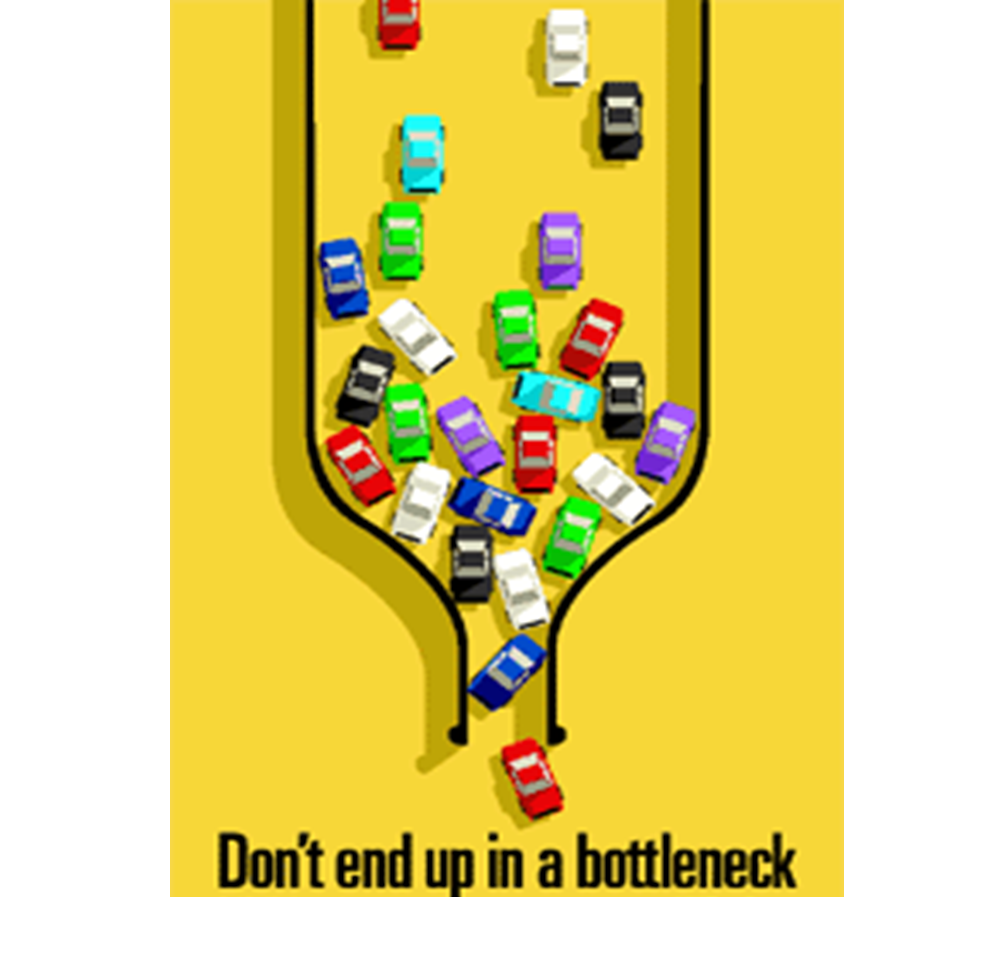
\includegraphics[scale=0.1]{bottleneck.png}

	Bottleneck : \textbf{{\huge Shared system context}}

\end{frame}

\begin{frame}
	\frametitle{Need for Replicas}
	For high availability, fault tolerance, performance and reliability of data
\end{frame}

\begin{frame}
	\frametitle{Consistency problem with replicas}
	CAP Theorem \footfullcite{gilbert2002brewer} and \\
	What is this PACELC \footfullcite{abadi2012consistency} (They say CAP is only part of the story)
	Pronounced pass-elk, it states that given there is a network \textbf{P}artition, then how does the system trades-off 	\textbf{A}vailability and \textbf{C}onsistency; \textbf{E}lse, in normal running condition how does the system trades-off 	\textbf{L}atency and \textbf{C}onsistency.

\end{frame}

\begin{frame}{Time, Clocks and Ordering of Events in Distributed Systems }

	CAP Theorem talks about necessity of ordering of events so that the bottleneck shared resource gets accessed one at a 	time in order.\\ They proved their theorem with \textbf{atomicity} and \textbf{linearizability}.

	Atomic and Linearizable  In CAP theorem paper Gilbert and Lynch say that, consistency guarantee means that operations on an atomic data object happen in a certain order such that each operation is completed at a single instant. 

\end{frame}

\begin{frame}
Partial ordering, Total ordering \footfullcite{lamport1978time}
\end{frame}

\subsection{Consistency Models}

\begin{frame}{Consistency has been defined?}
\begin{enumerate}
	\item Consistency by Relational database lens: ACID
\item Consistency by German scholars: The paper I am reading right now
\item Consistency by Sathish's suggestion: Paper: {\huge BASE}
\item Consistency how I understand: 
\end{enumerate}

\end{frame}



\begin{frame}{Base}
	I am reading the basically available , soft and eventually consistent consistency models.
Idea is to connect it all in the form of a story.\footfullcite{Pritchett2008}

\end{frame}




\section{Our Results/Contribution}

\subsection{Main Results}

\begin{frame}{Make Titles Informative.}
\end{frame}

\begin{frame}{Make Titles Informative.}
\end{frame}

\begin{frame}{Make Titles Informative.}
\end{frame}


\subsection{Basic Ideas for Proofs/Implementation}

\begin{frame}{Make Titles Informative.}

\end{frame}

\begin{frame}{Make Titles Informative.}
\end{frame}

\begin{frame}{Make Titles Informative.}
\end{frame}



\section*{Summary}

\begin{frame}{Summary}

  % Keep the summary *very short*.
  \begin{itemize}
  \item
    The \alert{first main message} of your talk in one or two lines.
  \item
    The \alert{second main message} of your talk in one or two lines.
  \item
    Perhaps a \alert{third message}, but not more than that.
  \end{itemize}
  
  % The following outlook is optional.
  \vskip0pt plus.5fill
  \begin{itemize}
  \item
    Outlook
    \begin{itemize}
    \item
      Something you haven't solved.
    \item
      Something else you haven't solved.
    \end{itemize}
  \end{itemize}
\end{frame}



% All of the following is optional and typically not needed. 
\appendix
\section<presentation>*{\appendixname}
\subsection<presentation>*{For Further Reading}

\begin{frame}[allowframebreaks]
  \frametitle<presentation>{For Further Reading}
    
  \begin{thebibliography}{10}
    
  \beamertemplatebookbibitems
  % Start with overview books.

  \bibitem{Author1990}
    A.~Author.
    \newblock {\em Handbook of Everything}.
    \newblock Some Press, 1990.
 
    
  \beamertemplatearticlebibitems
  % Followed by interesting articles. Keep the list short. 

  \bibitem{Someone2000}
    S.~Someone.
    \newblock On this and that.
    \newblock {\em Journal of This and That}, 2(1):50--100,
    2000.
  \end{thebibliography}
\end{frame}

\end{document}


